% Paper 4 manuscript. Built and checked by paper/tex/build_ms.py (gates G1-G8). Every number in the text is
% \V{key}{value} bound to a results file or a frozen document in paper/tex/bindings.json.
% Sources: paper/manuscript/introduction_draft.md and methods_draft.md (2026-11-10), PREREG_P4_draft.md (to be
% frozen; section numbers below refer to it). Journal not chosen yet (chosen after the results; criteria in the
% project HANDOFF): neutral article layout and source-style references until then. Results, Discussion and
% Abstract are \pending until the confirmatory runs (after the freeze).
\documentclass[11pt]{article}
\usepackage[a4paper,margin=25mm]{geometry}
\usepackage{fontspec}   % XeTeX (tectonic): Latin Modern OpenType, covers the Unicode in the reference strings
\usepackage{amsmath,amssymb}
\usepackage{graphicx}
\usepackage{booktabs}
\usepackage{textcomp}
\usepackage{caption}
\usepackage[hidelinks]{hyperref}
% Macros shared by main.tex and si.tex. The build gates (paper/tex/build_ms.py) read these names.
% \V{key}{value}  a number (math mode); key -> paper/tex/bindings.json; G1 compares value with the source
% \W{key}{word}   a count written as a word (text); same binding rules (fmt word / Word)
% \C{...}         a mathematical constant inside a formula (2 in 2 pi, 0 in p -> 0); no data
% \ID{...}        an identifier that contains digits (hash, date, version, DOI, ORCID, model-cell names); no data
% \snote{n}       a Supplementary Note number; G2 checks that si.tex defines it
% \pending{name}{text}  a result not yet available; G7 lists it and a --final build refuses it
\newcommand{\V}[2]{\ensuremath{#2}}
\newcommand{\W}[2]{#2}
\newcommand{\C}[1]{#1}
\newcommand{\ID}[1]{#1}
\newcommand{\snote}[1]{#1}
\newcommand{\pending}[2]{\par\noindent\fbox{\parbox{0.95\linewidth}{\textit{Pending result (#1).} #2}}\par}
\newcommand{\pss}{p/p_{\mathrm{sat}}}
\newcommand{\qref}{q_{\mathrm{ref}}}
\newcommand{\Qst}{Q_{\mathrm{st}}}

\newcommand{\kpp}{k''}
\newcommand{\RHf}{\mathrm{RH}_{\mathrm{flow}}}
\newcommand{\RHb}{\mathrm{RH}_{\mathrm{bed}}}
\newcommand{\RHh}{\mathrm{RH}_{50}}
\setlength{\emergencystretch}{1.5em}

\title{Does the isotherm predict an unseen sorbent's rate constant? A pre-registered held-out-sorbent test of
isotherm-driven water-uptake dynamics}
\author{Abdulhamid Batayhi\\ Department of Mechatronics Engineering, Faculty of Mechanical Engineering,\\ Yildiz
Technical University, \ID{34220} Istanbul, T\"urkiye\\ E-mail: abdulhamid.batayhi@std.yildiz.edu.tr}
\date{}

\begin{document}
\maketitle

\begin{abstract}
\pending{abstract}{Written after the confirmatory runs: question, design (pre-registered, held-out sorbents,
synthetic harnesses), the H4a$'$ verdict in its pre-registered wording, the harness record of the learned model, and
the error decomposition.}
\end{abstract}

\section*{Introduction}

Sorbents that take up and release water within minutes can be cycled many times a day, so their rate, and not only
their capacity, sets how much water a harvester or heat pump delivers. MOF-303 completes an adsorption--desorption
cycle within minutes under a mild temperature swing, which is what allows many harvesting cycles per
day~\cite{Hanikel2019Rapid}, and analyses of adsorption-based harvesting place heat and mass transport next to the
isotherm among the properties that set device output~\cite{LaPotin2019Adsorption}. Yet sorbents are usually
compared, and increasingly screened by machine learning, on equilibrium properties: the humidity of the
condensation step, the capacity and the cycling stability~\cite{Furukawa2014Water,Harriman2025Optimizing,
Alkhatib2026Machine,Zheng2023Shaping}. Whether the rate of a new sorbent can be predicted from the same equilibrium
data decides whether such screening can rank sorbents by what a cycle delivers.

The working models of sorption dynamics answer this with an assumption. They take the driving force from the
isotherm and lump everything else into a rate constant, in the linear-driving-force
tradition~\cite{Glueckauf1955Theory,Sircar2000Why} that adsorption-cooling and chiller models have long
used~\cite{Sakoda1984Fundamental,Chua2004Transient}. The approximation has known limits~\cite{Raymond2011Intraparticle},
and the measured rate depends on how the sorbent is held, as loose grains, glued grains or coatings, powder or
monolith~\cite{Solovyeva2023Water,Li2025Atmospheric}, and on loading within one framework~\cite{Hossain2019Kinetics}.
Bezrukov et al.\ measured the water uptake dynamics of seven MOFs and a silica gel by dynamic vapour sorption on
milligram powder layers and described them with one such model, in which the rate is proportional to the difference
between the humidity of the gas and the humidity in equilibrium with the current uptake, read from the isotherm,
with one rate constant for all materials~\cite{Bezrukov2023Regeneration}. If that holds, an unseen sorbent's
dynamics follow from its isotherm alone. The assumption was fitted to all sorbents together; it has not been tested
on a sorbent left out of the fit. Comparative studies of the same frameworks measure dynamics material by
material~\cite{Velte2023Adsorption,AbuElMaaty2024Kinetics}.
\pending{novelty}{Sentence on Xia et al.\ 2025 (structure--kinetics relationships of MOF water adsorption,
doi:10.1016/j.colsurfa.2025.137168) and the closing ``none asks whether an isotherm-based model predicts a sorbent it
has not seen'': written only after the full text has been read (metadata only so far).}

Learning offers an alternative. Hybrid models that place a neural network inside a mechanistic
equation~\cite{Psichogios1992Hybrid,Thompson1994Modeling}, now often written as universal differential
equations~\cite{Rackauckas2020Universal}, have been applied to adsorption
dynamics~\cite{Nogueira2022Using,Subraveti2022Physics}, and are expected to extrapolate better than black boxes
because the mechanistic part holds where data are lacking~\cite{Thompson1994Modeling}. Two cautions apply to any
claim that such a model transfers to new materials. Random splits overestimate performance on materials unlike those
in training, so a test must hold out whole materials or families~\cite{Meredig2018Can,Roberts2017Cross}, and leakage
between training and test data inflates results across machine-learning-based science~\cite{Kapoor2023Leakage}. And
a flexible model can appear to win for reasons that have nothing to do with the effect it is meant to capture;
testing a procedure on data simulated from a known truth, before it meets real data, is how such failures are
found~\cite{Cook2006Validation,Talts2018Validating}. With eight to ten materials the uncertainty of any hold-out score
is large~\cite{Varoquaux2018Cross}, which makes it all the more important that the analysis is fixed before the data
are seen~\cite{Nosek2018Preregistration}.

Here we test the isotherm-driven model on sorbents it has not seen, under a pre-registered protocol, and make three
contributions. First, a held-out-sorbent test of whether a learned grey-box correction, given only a sorbent's
isotherms, can be validated at all on data of this kind. Before real data, the model had to recover a known
correction in synthetic trajectories generated on the real humidity records and isotherms. It did so for two of three
held-out sorbents but not the third in its last allowed round, so under a stopping rule fixed in advance it was not
tested on real data, and we report its full record: leaving failed attempts out of the record biases what later
models learn from it~\cite{StriethKalthoff2022Machine}. Second, a confirmatory test, with its own synthetic harness
and a realistic-power check, of whether the isotherm of a held-out sorbent predicts the effective rate constant of
the published model better than one value shared by the training sorbents. Third, a decomposition of the published
model's error on unseen sorbents into the parts that a correct per-sorbent rate constant and a correct end point
would remove, and the cost of holding out a whole family.

\section*{Results}

\subsection*{The isotherm-driven model on unseen sorbents}

The study followed the order of Fig.~\ref{fig:workflow}. The primary set holds \V{n_seg}{1187} step segments in
\V{n_groups}{18} sorbent--temperature groups of eight sorbents and two composites, whose isotherms and step responses
differ widely (Fig.~\ref{fig:data}). Fitted on the training sorbents and evaluated on the held-out one, B0 left a
median error of \V{res_b0_lo}{0.055} to \V{res_b0_hi}{0.100} per fold under the primary dry-mass rule (Table~\ref{tab:h4a}),
\V{res_b0F_lo}{7} to \V{res_b0F_hi}{39} times the held-out sorbent's noise floor. In all \V{res_ncomp}{8} folds the
comparator chosen on the training sorbents was B0 with the adsorption branch in both directions; the
linear-driving-force model B1 was worse in every fold (median error \V{res_b1_lo}{0.12} to \V{res_b1_hi}{0.16}).

\subsection*{A learned correction could not be validated}

Before it could meet real data, the grey-box model L1 had to recover known corrections in synthetic trajectories
generated on the real humidity records and isotherms (Fig.~\ref{fig:harness}; Supplementary Table~S1). Over seven
rounds it came to recover $\kpp$ where no correction was present, with no false beat, and to beat B0 in the
correction worlds used during its development. In world C3, defined and committed before any run on it, it met every
condition on ROS-039 and on Al-fumarate (error ratios \V{res_ros_ratio}{0.36} and \V{res_alfu_ratio}{0.42}) but not
on MOF-303, where the injected effect was smallest: the median error fell from \V{res_mof_b0}{0.0128} to
\V{res_mof_l1}{0.0070}, but the gain was below the noise floor, the signed-rank $p$ was \V{res_mof_p}{0.034} and the
ratio \V{res_mof_ratio}{0.55} missed the required halving. Under the stopping rule written before that round, no
learned model passed the harness; H4a is therefore not tested, and no learned model was fitted to the real data. The
black-box model L2 had failed earlier, even without any correction to find, because an unconstrained flux network did
not hold the equilibrium over long plateaus (Supplementary Note~\snote{1}).

\subsection*{The isotherm does not predict the rate constant}

The harness of B2 passed all three of its criteria (Supplementary Note~\snote{2}): no fold was beaten without an
effect, all \V{res_Kbeats}{8} folds were beaten when the truth lay in B2's class, and \V{res_Sbeats}{3} of the
\V{res_nnull}{48} null fold-fits were beaten. On the real data B2 beat the pooled B0 in \V{res_beats_r2}{0} of the
\V{res_folds}{8} held-out folds under the primary rule and in \V{res_beats_r1}{0} under the sensitivity rule
(Fig.~\ref{fig:results}a, Table~\ref{tab:h4a}). No fold came near the practical margin: $r$ ranged from
\V{res_rmin_r2}{-10.9} to \V{res_rmax_r2}{1.6}\,\% under R2 and from \V{res_rmin_r1}{-10.6} to \V{res_rmax_r1}{3.9}\,\%
under R1, so the seventh order statistic of $r$, a one-sided \V{res_ub}{96.5}\,\% upper bound on its median, was
\V{res_o7_r2}{0.1}\,\% and \V{res_o7_r1}{2.0}\,\%. B2's median error was higher than B0's in
\V{res_worse_r2}{7} of the folds under R2 and \V{res_worse_r1}{5} under R1, and it beat B0 in neither non-trivial
family fold. H4a$'$ is falsified under both rules. Because B2 was supported in two of the three realistic-power worlds
of its harness, not all three, the pre-registered wording applies: no isotherm-predicted rate constant was detectable
at this noise and error level. The slopes fitted on the training sorbents also changed sign from fold to fold
(\V{res_bmin}{-0.61} to \V{res_bmax}{0.30} under R2), unlike the consistent slopes of the realistic-power and
form-error worlds (Supplementary Table~S2).

\subsection*{Where the error of the isotherm-driven model lies}

Fitting B0's rate constant on the held-out sorbent itself (B0$^{*}$, an oracle) closed \V{res_gap_lo}{-0.7} to
\V{res_gap_hi}{45}\,\% of the gap between B0 and the noise floor under R2, in no sorbent more than half, and lowered
B0's median error by \V{res_ownk_med}{15}\,\% at the median over sorbents (Fig.~\ref{fig:results}b). Scaling the
isotherm to the sorbent's own measured end points instead, with the pooled $\kpp$ unchanged, lowered B0's error in
\V{res_ep_n}{8} of the \V{res_ep_of}{8} folds, by \V{res_ep_lo}{3} to \V{res_ep_hi}{21}\,\% (median
\V{res_ep_med}{15}\,\%), and by more than a correct $\kpp$ did in \V{res_ep_beats}{3} of them. Under R1 the end point
helped in \V{res_ep_n_r1}{7} folds (median \V{res_ep_med_r1}{7}\,\%) and the oracle $\kpp$ closed up to
\V{res_gap_hi_r1}{50}\,\% of the gap. Neither oracle came close to the noise floor: the better of the two still left
at least \V{res_orF}{5.6} times $F$. Holding out a whole family raised B0's error for \V{res_h4c_r2}{5} of the
\V{res_h4c_n}{7} materials concerned under R2 (\V{res_h4c_r1}{3} under R1; Supplementary Table~S3).

\begin{table}[tbp]
\centering
\small
\caption{\textbf{H4a$'$ per held-out sorbent.} Relative improvement $r$ of B2 over the pooled B0 of the same variant
(the smaller per-material value in folds holding out a parent and its composite) under the primary (R2) and
sensitivity (R1) dry-mass rules, whether the fold was beaten by the pre-registered rule, the median held-out error of
B0, B2 and the oracle B0$^{*}$ (own $\kpp$) under R2, the share of the oracle's gain that B2 achieved (shown only where
the oracle improves on B0), and the temperatures (\textdegree C) at which the held-out descriptor lies outside the
training range.}
\label{tab:h4a}
% written by paper/tex/make_tables.py from results/confirm_R2|R1/decide.json and rows.jsonl; do not edit
\begin{tabular}{llccccccccc}
\toprule
 & & \multicolumn{2}{c}{$r$ (\%)} & \multicolumn{2}{c}{Beaten} & \multicolumn{3}{c}{Median $E$ (R2)} & & \\
\cmidrule(lr){3-4}\cmidrule(lr){5-6}\cmidrule(lr){7-9}
Held out & Variant & R2 & R1 & R2 & R1 & B0 & B2 & B0* & Share & Extrap.\\
\midrule
MOF-303 & B0 & $-0.3$ & $-1.2$ & no & no & 0.058 & 0.061 & 0.046 & $-0.32$ & --\\
MIL-160 & B0 & $-10.9$ & $3.9$ & no & no & 0.079 & 0.085 & 0.045 & $-0.19$ & --\\
CAU-10-H & B0 & $-3.3$ & $-10.6$ & no & no & 0.064 & 0.11 & 0.058 & $-8.79$ & 60\\
Al-fumarate & B0 & $-3.4$ & $2.0$ & no & no & 0.055 & 0.056 & 0.055 & $-3.73$ & 27\\
ROS-039 & B0 & $-5.0$ & $-3.3$ & no & no & 0.090 & 0.10 & 0.076 & $-0.80$ & 27, 60\\
ROS-040 & B0 & $1.6$ & $-0.2$ & no & no & 0.062 & 0.061 & 0.052 & $0.07$ & --\\
ROS-037 & B0 & $0.1$ & $0.0$ & no & no & 0.100 & 0.11 & 0.085 & $-0.39$ & --\\
Syloid AL-1 & B0 & $-0.3$ & $-0.1$ & no & no & 0.061 & 0.061 & 0.061 & -- & --\\
\bottomrule
\end{tabular}

\end{table}

\begin{figure}[tbp]
\centering
\makebox[\linewidth]{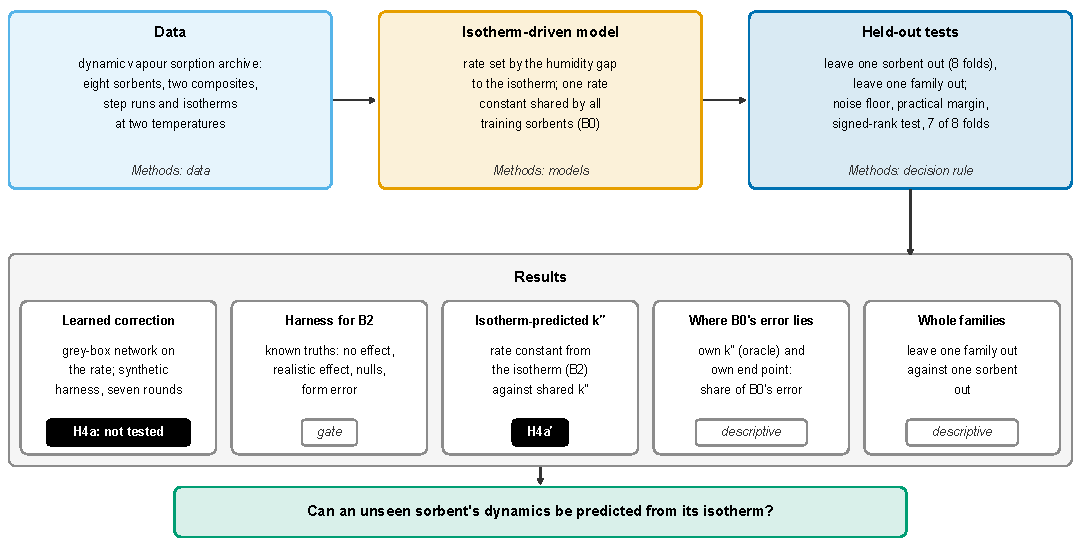
\includegraphics{../../figures/out/fig_workflow.pdf}}
\caption{\textbf{Workflow of the study.} Top: the data, the isotherm-driven model with one rate constant shared by
the training sorbents (B0), and the held-out tests with their decision rule. Middle: the result blocks; a black label
marks a pre-registered hypothesis with a decision rule, a white label a gate that must pass first or a descriptive
analysis. Bottom: the question the results answer. Schematic; no data.}
\label{fig:workflow}
\end{figure}

\begin{figure}[tbp]
\centering
\makebox[\linewidth]{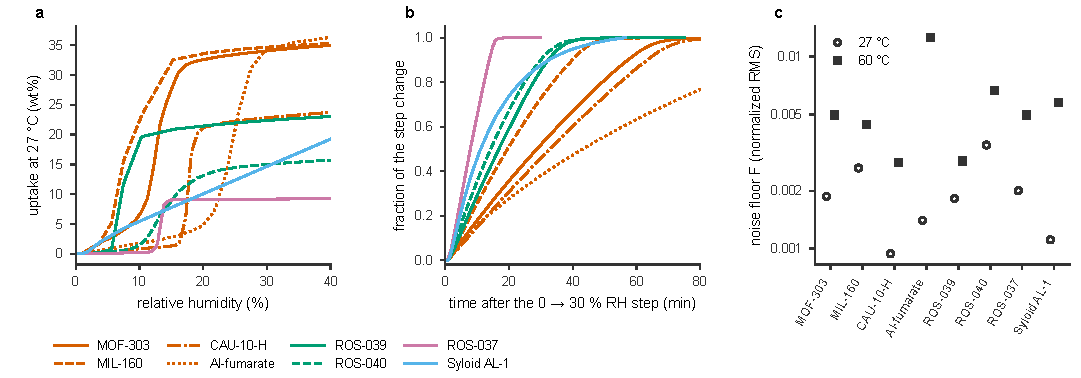
\includegraphics{../../figures/out/fig1_data.pdf}}
\caption{\textbf{The data.} \textbf{a}, Adsorption isotherms of the eight sorbents at \V{T_lo}{27}~\textdegree C.
\textbf{b}, Normalised uptake after the step from \V{rh_lo}{0} to \V{rh_hi}{30}\,\% RH at \V{T_lo2}{27}~\textdegree C.
\textbf{c}, Noise floor $F$, the normalised RMS difference between consecutive repeats of the same step, per sorbent
and temperature.}
\label{fig:data}
\end{figure}

\begin{figure}[tbp]
\centering
\makebox[\linewidth]{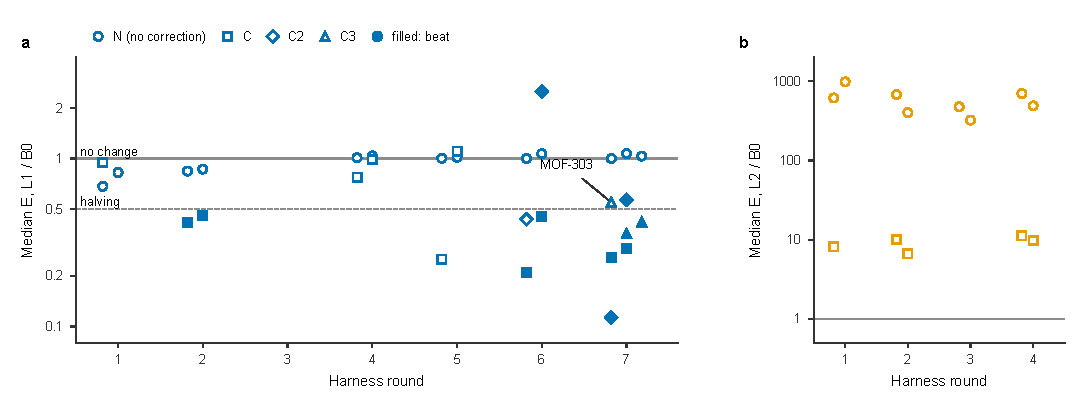
\includegraphics{../../figures/out/fig_harness_l1.pdf}}
\caption{\textbf{Synthetic harness record of the learned models} (synthetic data only). \textbf{a}, Grey box L1:
median held-out error of L1 over that of B0 refitted on the training sorbents, per harness round, world and held-out
sorbent; marker shape gives the world (N, no correction; C, C2, C3, correction worlds), a filled marker a beat by
the rule in force in that round. Lines mark no change and the halving required from round~\ID{3}. \textbf{b}, Black
box L2, rounds \ID{1} to \ID{4}, dropped after round~\ID{4}.}
\label{fig:harness}
\end{figure}

\begin{figure}[tbp]
\centering
\makebox[\linewidth]{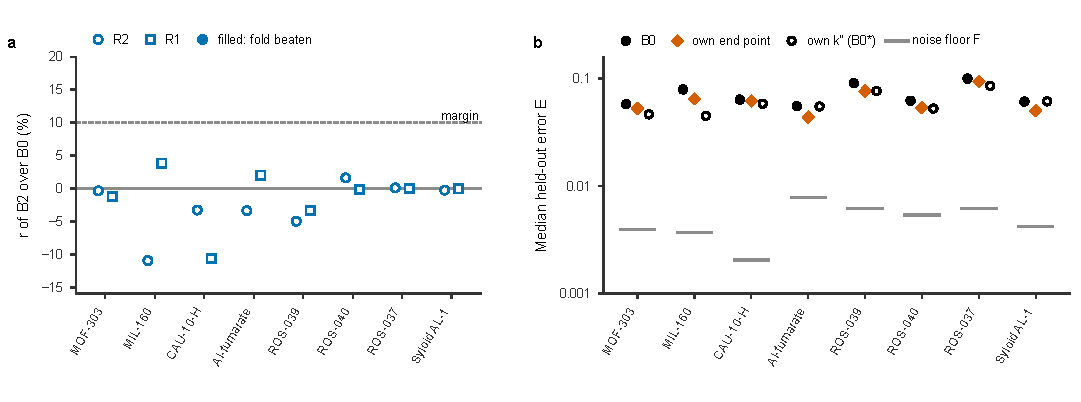
\includegraphics{../../figures/out/fig_results.pdf}}
\caption{\textbf{Confirmatory result.} \textbf{a}, Relative improvement $r$ of B2, the isotherm-predicted rate
constant, over the pooled B0 per held-out sorbent under the primary (R2, circles) and sensitivity (R1, squares)
dry-mass rules; a filled marker would mark a fold beaten by the pre-registered rule (none was). The dashed line is the
\V{fig_margin}{10}\,\% practical margin. \textbf{b}, Median held-out error of B0, of B0 with the sorbent's own end
point, and of B0 with its own rate constant (B0$^{*}$), with the sorbent's noise floor $F$ (bar), under R2.}
\label{fig:results}
\end{figure}

\section*{Discussion}

\pending{discussion}{After the results: what the verdict means for screening by isotherm, the error decomposition,
limits (powder layers in one instrument, eight sorbents, effective rate constant only), and what a test of a
learned model would need.}

\section*{Methods}

\subsection*{Pre-registration and order of events}

The protocol was written before any model was fitted to held-out real data and frozen on \ID{2026-11-11} at commit
\ID{bf0b2cf} (tag \texttt{prereg-p4-freeze}; hashes of the protocol, code and derived data in its freeze manifest);
every change before the freeze is listed with its cause in the protocol's
corrections section. The order of events matters for how the results may be read. The original primary hypothesis,
H4a, asked whether a learned model, given only an unseen sorbent's isotherms, predicts its uptake trajectories better
than the published isotherm-driven model. A learned model could enter that test only after passing a synthetic
ground-truth harness. The grey-box model L1 failed the harness in its last allowed round, under a stopping rule
written before that round's judged result existed, so H4a is reported as not tested and no learned model was fitted
to the real data. The confirmatory hypothesis H4a$'$ was then added, before any fit of its model to held-out real
data; that model's form had been fixed two days earlier, on \ID{2026-11-08}, as a reported comparator (commit
\ID{127ab6d}). H4a$'$ has its own harness, which had to pass before the freeze.

\subsection*{Data}

We used the dynamic vapour sorption (DVS) archive of Bezrukov et al.~\cite{Bezrukov2023Regeneration,Bezrukov2023Data},
deposited under a CC~BY~\ID{4.0} licence. It holds step runs, cycling runs and isotherms of \W{n_sorbents}{eight}
sorbents: MOF-303, MIL-160, CAU-10-H and Al-fumarate (aluminium carboxylate rods), ROS-039 and ROS-040 (zinc
triazolate fluorides), ROS-037 (a copper framework) and the silica gel Syloid AL-1, plus composites of ROS-037 and
ROS-039. The primary set contains all step runs at \V{T_a}{27} and \V{T_b}{60}~\textdegree C, all
\V{cyc_lo}{0}--\V{cyc_hi}{30}\,\% RH cycling runs at \V{T_cyc}{27}~\textdegree C and the isotherms at both
temperatures; particle-size, packing, pan and flow variations and the long cycling runs are reserved for secondary
analyses. \W{n_dup}{Eight} files duplicate another file's mass trace exactly; the copy in the sorbent's main folder
is kept.

Uptake is $w = \C{100}\,(m - m_{\mathrm{dry}})/m_{\mathrm{dry}}$ in wt\%. The instrument's reference mass is not
used, because the sample is not yet dry when it is recorded. The primary dry mass (rule R2) is the median mass over
the last minute of the unheated \V{rh_dry}{0}\,\% RH stretch that follows the heated activation
(\V{r2_lo}{70} to \V{r2_hi}{229}~min, median \V{r2_med}{90}). It was chosen because the mass has stopped changing
there: the median drift over the last \V{drift_win}{10}~min is \V{drift_r2}{0.023}\,\%\,h$^{-1}$, against
\V{drift_r1}{0.106}\,\%\,h$^{-1}$ at the end of the heated activation (rule R1; \V{drift_n}{80} runs each). Every
confirmatory result is computed under both rules, and a verdict stands only if both give it. The composites' step
runs at \V{T_comp}{27}~\textdegree C, dried only at that temperature and still losing \V{comp_lo}{0.3} to
\V{comp_hi}{0.9}\,\% of their mass per hour, and all cycling runs, which have no drying stage, are excluded from the
confirmatory comparisons. Models are driven by the measured humidity, the sample temperature and the sample's dry
mass, and are told nothing about the held-out sorbent except its adsorption and desorption isotherms at both
temperatures. Trajectories are resampled to a \V{grid}{6}~s grid, which keeps at least \V{grid_pts}{11} points within
the fastest time to \V{t63}{63}\,\% of a step (\V{t63_min}{1.1}~min).

\subsection*{Units, folds and clusters}

The unit of evaluation is a step segment, one humidity plateau of a step run, simulated open loop from the measured
uptake at its first grid point. \W{n_loso}{Eight} leave-one-sorbent-out (LOSO) folds hold out each sorbent, a
composite always together with its parent. Two leave-one-family-out (LOFO) folds hold out the aluminium rods and the
zinc triazolates; the other two family folds coincide with LOSO folds. Everything fitted is fitted on the training
sorbents only.

Two pans measured together share their forcing, and each sorbent was measured in few sessions. The inference cluster
is therefore one humidity step (from-RH, to-RH) in one session, averaging both pans and all repeats; a material has
\V{clu_lo}{13} to \V{clu_hi}{54} clusters. A per-fold result is a consistency check over humidity conditions for the
samples measured; the claim about unseen sorbents rests on the count over folds.

\subsection*{Models}

B0 is Bezrukov's model~\cite{Bezrukov2023Regeneration},
\begin{equation}
\frac{\mathrm{d}w}{\mathrm{d}t} = \frac{\kpp}{m}\,\bigl(\RHf - \RHb(w)\bigr),
\end{equation}
with $\RHb(w)$ the inverse of the held-out sorbent's adsorption isotherm and one $\kpp$ for uptake and one for
release at each temperature, shared by all training sorbents. B0-b reads the desorption branch during release, and
B1 is a linear-driving-force model, $\mathrm{d}w/\mathrm{d}t = (k'''/m)\,(w^{*}(\RHf) - w)$. The comparator
candidates have the same four parameters. All physics models are fitted by the scored metric (the median normalised
error over segments, below) rather than by least squares, so that no model gains merely from being fitted to the
metric it is scored on.

B2, the model of H4a$'$, is B0 with an isotherm-predicted rate constant,
\begin{equation}
\log \kpp = a + b\,(x - \bar{x}), \qquad x = \RHh / 30\,\%,
\end{equation}
where $\RHh$ is the humidity at which the adsorption branch reaches half its uptake at \V{rh50_ref}{30}\,\% RH and
$\bar{x}$ the mean of $x$ over the training sorbents; $a$ and $b$ are fitted for each temperature and direction.
$\RHh$ spans \V{rh50_27_lo}{7.4} to \V{rh50_27_hi}{24.3}\,\% RH at \V{T_r1}{27}~\textdegree C and
\V{rh50_60_lo}{10.5} to \V{rh50_60_hi}{28.7}\,\% RH at \V{T_r2}{60}~\textdegree C. B2 is built on the fold's B0
variant, so that it differs from the pooled model in $\kpp$ alone. The oracle B0$^{*}$ is B0 with $\kpp$ fitted on
the held-out sorbent's own data; it is not a competitor but measures what any single per-sorbent $\kpp$ could gain.

The learned grey-box model L1 multiplied B0's rate by a bounded positive factor, $\exp(\C{2}\tanh g_\theta(z))$,
from a small network of local isotherm features and the driving force, so that the rate stays zero at equilibrium.
It is described in full with its harness record in the Supplementary Information.

\subsection*{Metric and noise floor}

The error of a segment is $E = \mathrm{RMS}(w_{\mathrm{pred}} - w_{\mathrm{meas}})/|\Delta w|$, with $\Delta w$ the
measured change over the segment. The noise floor $F$ of a material is the median error between consecutive repeats
of the same step within one file, aligned on time since the step, as a segment-weighted mean over its two
temperatures; $F$ is \V{F_lo}{0.0021} to \V{F_hi}{0.0078}.

\subsection*{Decision rule}

For each held-out material, $d = E_{\mathrm{B0}} - E_{\mathrm{B2}}$ per segment and $D = d\,|\Delta w|$ are averaged
within clusters. B2 beats B0 on a material if (\C{1}) the median cluster $d$ exceeds that material's $F$; (\C{2}) the
relative improvement $r$, the median $d$ over B0's median cluster $E$, is at least \V{margin}{10}\,\%; (\C{3}) a
one-sided exact Wilcoxon signed-rank test of $D$ over clusters gives $p \le \V{alpha}{0.025}$; and (\C{4}) B2's median
cluster $E$
is below B0's. A fold is beaten if every held-out material is beaten and B2's excess physical violations (uptake
moving against the step by more than \V{viol_w}{0.05}~wt\% within a minute, on segments where neither the data nor B0
do so) stay at or below \V{viol_frac}{5}\,\% of the fold's segments. H4a$'$ is supported if at least
\V{need}{7} of the \V{nfold}{8} LOSO folds are beaten, falsified if at most one fold has $r \ge \V{margin2}{10}\,\%$
(the seventh order statistic of $r$ is then a one-sided \V{ub}{96.5}\,\% upper bound on its median, below
\V{margin3}{10}\,\%), and not established otherwise. The verdict must agree under R1 and R2, and the B2 harness must
have passed, or H4a$'$ is not tested. The \V{margin4}{10}\,\% margin was proposed after the noise floor and an
in-sample reproduction of B0 were seen and before any learned model was fitted to real data.

\subsection*{Synthetic harnesses}

Both harnesses generate trajectories on the real forcing, isotherms and dry masses from a known truth, add
autocorrelated noise ($\sigma = \V{sigma}{0.01}$~wt\%, $\varphi = \V{phi}{0.9}$), and run the confirmatory pipeline.
For L1 the harness required recovery of $\kpp$ in a world without correction, a beat and a halving of B0's error in a
correction world not used during development, and no false positive; it ran in seven rounds, with the judging world
replaced whenever a world had been used for diagnosis, and stopped by rule after round~\ID{7}. For B2 the harness
(version~\ID{2}, commit \ID{78accf6}) has a world without effect, a plumbing world whose truth lies in B2's class,
three realistic-power worlds with the effect at the measured size of the across-sorbent spread of $\kpp$ plus
end-point offsets, six structure-free null worlds with sorbent-level rate and end-point deviations independent of the
isotherm, and a form-error world. Its pass criteria and the role of each world are given in the Supplementary
Information.

\subsection*{Descriptive analyses}

H4b reports, per held-out sorbent, the fraction of the gap between B0 and $F$ that the oracle B0$^{*}$ closes; an
in-sample version was seen before the freeze. An end-point oracle re-scores B0 with its isotherm scaled by the
held-out sorbent's own equilibrium offset, estimated from its equilibrated segments that end where the adsorption
uptake is at least \V{eps_thr}{0.2} of the uptake at \V{eps_rh}{30}\,\% RH. Together the two oracles separate the part
of B0's error that a correct end point removes from the part that a correct $\kpp$ removes. H4c compares LOSO and
family-level errors without a test.

\section*{Data Availability}

\pending{availability}{Repository and Zenodo DOI of the code, pre-registration, harness records and every results
file; the raw data stay at their source (Zenodo, doi:10.5281/zenodo.6631711; CC~BY~4.0).}

\section*{Author Contributions}

A.B.: conceptualization, methodology, software, formal analysis, data curation, visualization, writing (original draft,
review and editing).

\section*{Conflicts of Interest}

There are no conflicts to declare.

\section*{Use of Generative AI}

During the preparation of this work the author used a generative AI assistant (Claude, Anthropic) as a tool to assist
with drafting and language editing, with writing and checking code, and with checking bibliographic records. The
author designed the study, made every scientific decision, reviewed and edited all content, and takes full
responsibility for the content of the published article.

\section*{Acknowledgements}

The author thanks Bezrukov et al.\ for depositing their complete measurement archive under an open licence. This work
received no specific grant.

% written by build_ms.py from refs_master.json (order of first citation); do not edit
\renewcommand\refname{References}
\begin{thebibliography}{99}
\bibitem{Hanikel2019Rapid} Hanikel, N., Prévot, M. S., Fathieh, F., Kapustin, E. A., Lyu, H., Wang, H., Diercks, N. J., Glover, T. G. \& Yaghi, O. M. Rapid Cycling and Exceptional Yield in a Metal-Organic Framework Water Harvester. \textit{ACS Central Science} \textbf{5}, 1699 (2019). doi:10.1021/acscentsci.9b00745
\bibitem{LaPotin2019Adsorption} LaPotin, A., Kim, H., Rao, S. R. \& Wang, E. N. Adsorption-Based Atmospheric Water Harvesting: Impact of Material and Component Properties on System-Level Performance. \textit{Accounts of Chemical Research} \textbf{52}, 1588 (2019). doi:10.1021/acs.accounts.9b00062
\bibitem{Furukawa2014Water} Furukawa, H., Gándara, F., Zhang, Y.-B., Jiang, J., Queen, W. L., Hudson, M. R. \& Yaghi, O. M. Water Adsorption in Porous Metal–Organic Frameworks and Related Materials. \textit{Journal of the American Chemical Society} \textbf{136}, 4369 (2014). doi:10.1021/ja500330a
\bibitem{Harriman2025Optimizing} Harriman, C., Ke, Q., Vlugt, T. J. H., Howarth, A. J. \& Simon, C. M. Optimizing Mixtures of Metal–Organic Frameworks for Robust and Bespoke Passive Atmospheric Water Harvesting. \textit{ACS Engineering Au} \textbf{5}, 707 (2025). doi:10.1021/acsengineeringau.5c00051
\bibitem{Alkhatib2026Machine} Alkhatib, N., Abed Alrhman, S. \& Kirmizialtin, S. Machine learning highlights chemistry as the key factor in metal–organic frameworks for atmospheric water harvesting. \textit{Molecular Systems Design \& Engineering} \textbf{11}, 50 (2026). doi:10.1039/D5ME00101C
\bibitem{Zheng2023Shaping} Zheng, Z., Alawadhi, A. H., Chheda, S., Neumann, S. E., Rampal, N., Liu, S., Nguyen, H. L., Lin, Y.-h., Rong, Z., Siepmann, J. I., Gagliardi, L., Anandkumar, A., Borgs, C., Chayes, J. T. \& Yaghi, O. M. Shaping the Water-Harvesting Behavior of Metal–Organic Frameworks Aided by Fine-Tuned GPT Models. \textit{Journal of the American Chemical Society} \textbf{145}, 28284 (2023). doi:10.1021/jacs.3c12086
\bibitem{Glueckauf1955Theory} Glueckauf, E. Theory of chromatography. Part 10.—Formulæ for diffusion into spheres and their application to chromatography. \textit{Trans. Faraday Soc.} \textbf{51}, 1540 (1955). doi:10.1039/TF9555101540
\bibitem{Sircar2000Why} Sircar, S. \& Hufton, J. R. Why Does the Linear Driving Force Model for Adsorption Kinetics Work? \textit{Adsorption} \textbf{6}, 137 (2000). doi:10.1023/A:1008965317983
\bibitem{Sakoda1984Fundamental} SAKODA, A. \& SUZUKI, M. Fundamental study on solar powered adsorption cooling system. \textit{JOURNAL OF CHEMICAL ENGINEERING OF JAPAN} \textbf{17}, 52 (1984). doi:10.1252/jcej.17.52
\bibitem{Chua2004Transient} Chua, H. T., Ng, K. C., Wang, W., Yap, C. \& Wang, X. L. Transient modeling of a two-bed silica gel–water adsorption chiller. \textit{International Journal of Heat and Mass Transfer} \textbf{47}, 659 (2004). doi:10.1016/j.ijheatmasstransfer.2003.08.010
\bibitem{Raymond2011Intraparticle} Raymond, A. \& Garimella, S. Intraparticle Mass Transfer in Adsorption Heat Pumps: Limitations of the Linear Driving Force Approximation. \textit{Journal of Heat Transfer} \textbf{133}, 042001 (2011). doi:10.1115/1.4001310
\bibitem{Solovyeva2023Water} Solovyeva, M. \& Gordeeva, L. Water Adsorption Dynamics on Metal–Organic Framework MOF-801: Comparative Study of Loose and Glued Grains, and Coatings. \textit{Nanomaterials} \textbf{13}, 2442 (2023). doi:10.3390/nano13172442
\bibitem{Li2025Atmospheric} Li, J., Wang, G., Fan, H., Li, Z., Tso, C. Y. \& Zhou, Y. Atmospheric Water Sorption Kinetics in Powder and Monolithic Metal–Organic Frameworks. \textit{Advanced Materials Interfaces} \textbf{12}, 2400628 (2025). doi:10.1002/admi.202400628
\bibitem{Hossain2019Kinetics} Hossain, M. I. \& Glover, T. G. Kinetics of Water Adsorption in UiO-66 MOF. \textit{Industrial \& Engineering Chemistry Research} \textbf{58}, 10550 (2019). doi:10.1021/acs.iecr.9b00976
\bibitem{Bezrukov2023Regeneration} Bezrukov, A. A., O’Hearn, D. J., Gascón-Pérez, V., Darwish, S., Kumar, A., Sanda, S., Kumar, N., Francis, K. \& Zaworotko, M. J. Metal-organic frameworks as regeneration optimized sorbents for atmospheric water harvesting. \textit{Cell Reports Physical Science} \textbf{4}, 101252 (2023). doi:10.1016/j.xcrp.2023.101252
\bibitem{Velte2023Adsorption} Velte, A., Laurenz, E., Rustam, L., P.C. Hügenell, P., Henninger, M., Seiler, J. \& Füldner, G. Adsorption dynamics and hydrothermal stability of MOFs aluminium fumarate, MIL-160 (Al), and CAU-10-H, and zeotype TiAPSO for heat transformation applications. \textit{Applied Thermal Engineering} \textbf{227}, 120336 (2023). doi:10.1016/j.applthermaleng.2023.120336
\bibitem{AbuElMaaty2024Kinetics} Abu EL-Maaty, A. E., Abdalla, M. A., Essalhi, M., Abdelnaby, M. M., Mahmoud, M. M., Habib, M. A., Antar, M. \& Ben-Mansour, R. Kinetics of Water Adsorption in Metal-Organic Framework(MOF-303) for Adsorption Cooling Application. \textit{Energy Conversion and Management: X} \textbf{24}, 100694 (2024). doi:10.1016/j.ecmx.2024.100694
\bibitem{Psichogios1992Hybrid} Psichogios, D. C. \& Ungar, L. H. A hybrid neural network‐first principles approach to process modeling. \textit{AIChE Journal} \textbf{38}, 1499 (1992). doi:10.1002/aic.690381003
\bibitem{Thompson1994Modeling} Thompson, M. L. \& Kramer, M. A. Modeling chemical processes using prior knowledge and neural networks. \textit{AIChE Journal} \textbf{40}, 1328 (1994). doi:10.1002/aic.690400806
\bibitem{Rackauckas2020Universal} Rackauckas, C., Ma, Y., Martensen, J., Warner, C., Zubov, K., Supekar, R., Skinner, D., Ramadhan, A. \& Edelman, A. Universal Differential Equations for Scientific Machine Learning. Preprint at arXiv:2001.04385 (2020). doi:10.48550/arXiv.2001.04385
\bibitem{Nogueira2022Using} B. R. Nogueira, I., V. Santana, V., Ribeiro, A. M. \& Rodrigues, A. E. Using scientific machine learning to develop universal differential equation for multicomponent adsorption separation systems. \textit{The Canadian Journal of Chemical Engineering} \textbf{100}, 2279 (2022). doi:10.1002/cjce.24495
\bibitem{Subraveti2022Physics} Subraveti, S. G., Li, Z., Prasad, V. \& Rajendran, A. Physics-Based Neural Networks for Simulation and Synthesis of Cyclic Adsorption Processes. \textit{Industrial \& Engineering Chemistry Research} \textbf{61}, 4095 (2022). doi:10.1021/acs.iecr.1c04731
\bibitem{Meredig2018Can} Meredig, B., Antono, E., Church, C., Hutchinson, M., Ling, J., Paradiso, S., Blaiszik, B., Foster, I., Gibbons, B., Hattrick-Simpers, J., Mehta, A. \& Ward, L. Can machine learning identify the next high-temperature superconductor? Examining extrapolation performance for materials discovery. \textit{Molecular Systems Design \& Engineering} \textbf{3}, 819 (2018). doi:10.1039/C8ME00012C
\bibitem{Roberts2017Cross} Roberts, D. R., Bahn, V., Ciuti, S., Boyce, M. S., Elith, J., Guillera‐Arroita, G., Hauenstein, S., Lahoz‐Monfort, J. J., Schröder, B., Thuiller, W., Warton, D. I., Wintle, B. A., Hartig, F. \& Dormann, C. F. Cross‐validation strategies for data with temporal, spatial, hierarchical, or phylogenetic structure. \textit{Ecography} \textbf{40}, 913 (2017). doi:10.1111/ecog.02881
\bibitem{Kapoor2023Leakage} Kapoor, S. \& Narayanan, A. Leakage and the reproducibility crisis in machine-learning-based science. \textit{Patterns} \textbf{4}, 100804 (2023). doi:10.1016/j.patter.2023.100804
\bibitem{Cook2006Validation} Cook, S. R., Gelman, A. \& Rubin, D. B. Validation of Software for Bayesian Models Using Posterior Quantiles. \textit{Journal of Computational and Graphical Statistics} \textbf{15}, 675 (2006). doi:10.1198/106186006X136976
\bibitem{Talts2018Validating} Talts, S., Betancourt, M., Simpson, D., Vehtari, A. \& Gelman, A. Validating Bayesian Inference Algorithms with Simulation-Based Calibration. Preprint at arXiv:1804.06788 (2018). doi:10.48550/arXiv.1804.06788
\bibitem{Varoquaux2018Cross} Varoquaux, G. Cross-validation failure: Small sample sizes lead to large error bars. \textit{NeuroImage} \textbf{180}, 68 (2018). doi:10.1016/j.neuroimage.2017.06.061
\bibitem{Nosek2018Preregistration} Nosek, B. A., Ebersole, C. R., DeHaven, A. C. \& Mellor, D. T. The preregistration revolution. \textit{Proceedings of the National Academy of Sciences} \textbf{115}, 2600 (2018). doi:10.1073/pnas.1708274114
\bibitem{StriethKalthoff2022Machine} Strieth‐Kalthoff, F., Sandfort, F., Kühnemund, M., Schäfer, F. R., Kuchen, H. \& Glorius, F. Machine Learning for Chemical Reactivity: The Importance of Failed Experiments. \textit{Angewandte Chemie International Edition} \textbf{61}, e202204647 (2022). doi:10.1002/anie.202204647
\bibitem{Bezrukov2023Data} Bezrukov, A. A., O'Hearn, D. J., Gascón-Pérez, V., Darwish, S., Kumar, A., Sanda, S., Kumar, N., Francis, K. \& Zaworotko, M. J. Metal-organic frameworks as regeneration optimized sorbents for atmospheric water harvesting. \textit{Zenodo} (2023). doi:10.5281/zenodo.6631711
\end{thebibliography}


\end{document}
